% ========================================
% Preamble
% - Type of document: define class, set margin
% - Package and pre-define
% ========================================



                                        % ========================================
                                        % [Type doctument]
                                        %   document type
                                        %       - \documentclass[option]{class}
                                        %   margin
                                        %       - geometry: set margin, paper should
                                        %           similar with \documentclass
                                        % ========================================
                    % Document type
\documentclass[12pt, a4paper, twoside]{report}
                    % Margin
\usepackage[a4paper,inner=3cm,outer=2cm, top=2cm, bottom=2.5cm]{geometry}



                                        % ========================================
                                        % [Package and pre-define]
                                        %   Template paragraphs
                                        %       - lipsum: lorem paragraph
                                        %   Language and format document
                                        %       - inputenc: input encoder
                                        %       - fontenc:  font encoder
                                        %           T1 for ENG, T5 for VIE, ...
                                        %       - lmodern: Latin modern font 
                                        %           (vector base on Computer Modern) 
                                        %       - babel: re-translate section suitable
                                        %           with requiring language, and handle
                                        %           where should hyphenate text
                                        %   Url / reference
                                        %       - hyperref: hide and onclick url
                                        %       - xurl: fix url can't slice
                                        %   Color
                                        %       - color / xcolor: supply more color
                                        %   Table / figure
                                        %       - array: expand ability align text 
                                        %           for tabular
                                        %       - graphicx: draw image, resize box, ...
                                        %       - rotating: rotate static environment
                                        %       - rotfloat: prerequisite `rotating'
                                        %           help rotate a float environment
                                        %       - float: expand option `H' - here absolute
                                        %   Mathematic
                                        %       - mathtools: include amsmath
                                        %           supply math symbol and math environment
                                        %       - amssymb: expand math symbols
                                        %   Source code
                                        %       - listings: varity highlight code type 
                                        %           and support line numbering
                                        %   Background and foregroud
                                        %       - eso-pic: design for 1 or all pages
                                        %   TOC, LOT, LOF style
                                        %       - tocloft: 
                                        %   Abbrivication part
                                        %       - nomencl: make nomenclature table
                                        %   Glossary part
                                        %       - glossaries: make glossaries information
                                        %           for the concepts in document
                                        %   Index part:
                                        %       - makeidx
                                        %   Basic calculator
                                        %       - calc: + - * /
                                        %           group by `()'
                                        %   Basic graphic command
                                        %       - tikz: draw yourself
                                        % ========================================
                    % Template paragraphs
\usepackage{lipsum}
                    % Language and format document
\usepackage[utf8]{inputenc}
% fontenc auto change font 
% encoder in list of order 
% if current encoder not available
\usepackage[T1, T5]{fontenc} 
\usepackage{lmodern}
% babel default choose last
% vietnam last -> default 
\usepackage[english, vietnamese]{babel} 
% \usepackage[vietnamese,english]{babel} 
                    % Url / reference
\usepackage[hidelinks]{hyperref}
\usepackage{xurl}
                    % Color
\usepackage[table]{xcolor}
                    % Table / figure
\usepackage{array}
\usepackage{graphicx}
\usepackage{rotating}
\usepackage{rotfloat}
\usepackage{float}                    
                    % Mathematic
\usepackage{mathtools}
\usepackage{amssymb}
                    % Source code
\usepackage{listings}
                    % Background and foregroud
\usepackage{eso-pic}
                    % TOC, LOT, LOF style
\usepackage{tocloft}
                    % Abbrivication part
\usepackage{nomencl}
\makenomenclature
\renewcommand{\nomname}{Danh mục ký hiệu và chữ viết tắt}
                    % Glossary part
\usepackage{glossaries}
\makeglossaries
% \renewcommand{\glossaryname}{Terminology}
                    % Index part
\usepackage{makeidx}
\makeindex
% \renewcommand{\indexname}{Alphabetical Index}
                    % Basic Calculator
\usepackage{calc}
                    % Basic graphic command
\usepackage{tikz}
% ========================================
% Main Document
% ========================================
\begin{document}



                                        % ========================================
                                        % [Predefine]
                                        %   - Glossary definitions
                                        %   - Page style
                                        % ========================================



                    % ========================================
                    % [Definitions of Glossary]
                    %   - Classify definitions of glossaries 
                    %       into `.tex' and include here
                    % ========================================
                    % Lib 1: Topic ...
% \input{./gl_01.tex}
                    % Lib 2: Topic ...
% \input{./gl_02.tex}

% % has to at least 1 entry
% \newglossaryentry{qt}{
%     name={Qt},
%     description={A cross-platform application framework}
% }



                    % ========================================
                    % [Design page style]
                    % ========================================
% `footer' blank, `header' show section and page number
\pagestyle{headings}
% defaut background and foreground
\AddToShipoutPictureBG*
{
    % offset image width


    % upper right
    \put(\paperwidth - \paperwidth*1/5, \paperheight - \paperheight*1/5)
    {
        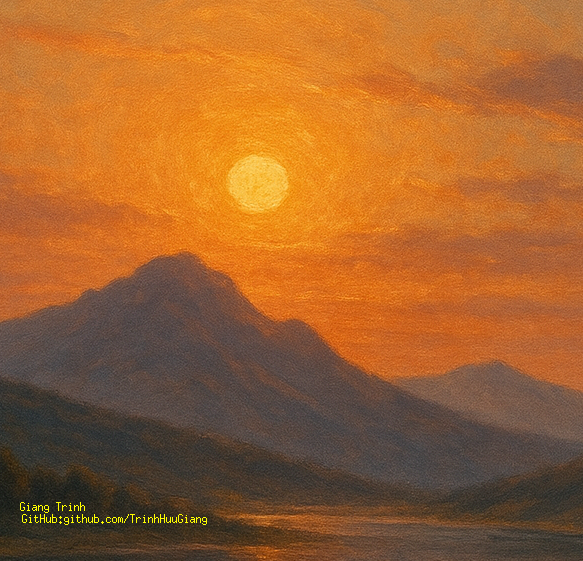
\includegraphics
        [width=\paperwidth*1/5,height=\paperheight*1/5,keepaspectratio=false]
        {sunset.png}
    }
    % upper left
    \put(0pt, \paperheight - \paperheight*1/5)
    {
        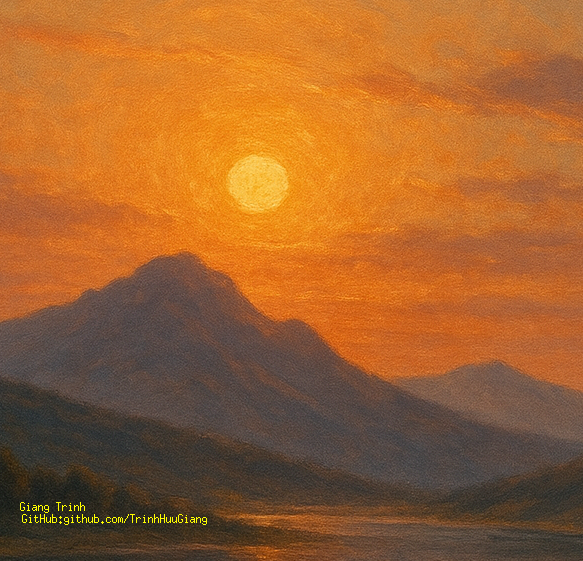
\includegraphics
        [width=\paperwidth*1/5,height=\paperheight*1/5,keepaspectratio=false]
        {sunset.png}
    }
    % lower right
    \put(\paperwidth - \paperwidth*1/5, 0pt)
    {
        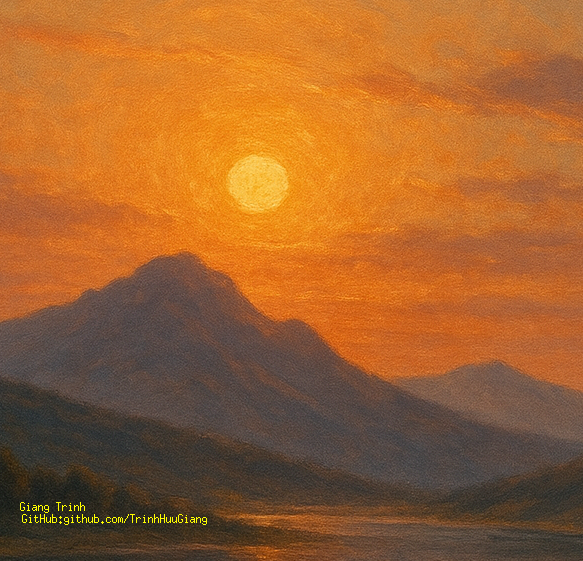
\includegraphics
        [width=\paperwidth*1/5,height=\paperheight*1/5,keepaspectratio=false]
        {sunset.png}
    }
    % lower left
    \put(0 , 0)
    {
        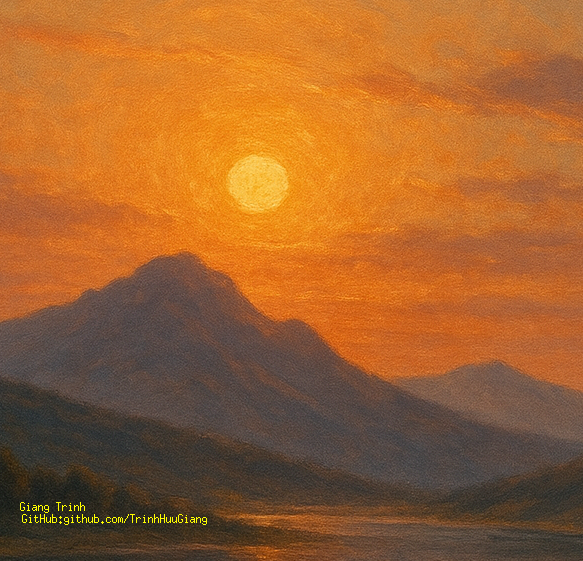
\includegraphics[width=\paperwidth*1/5,height=\paperheight*1/5,keepaspectratio=false]{sunset.png}
    }

    % Test some tikz
    \put(5cm, 5cm)
    {
        \begin{tikzpicture}
            \tikz \draw[thick,rounded corners=8pt]
            (0,0) -- (0,2) -- (1,3.25) -- (2,2) -- (2,0) -- (0,2) -- (2,2) -- (0,0) -- (2,0);
        \end{tikzpicture}
    }

}



                                        % ========================================
                                        % [Pront matter]
                                        %   - title, information, dedication,
                                        %   - TOC, abbreviation, LOT, LOF
                                        %   - preface, abstract
                                        % ========================================
% \frontmatter % only for book



                    % ========================================
                    % [Drawing title page]
                    % ========================================
% title
\title
{
    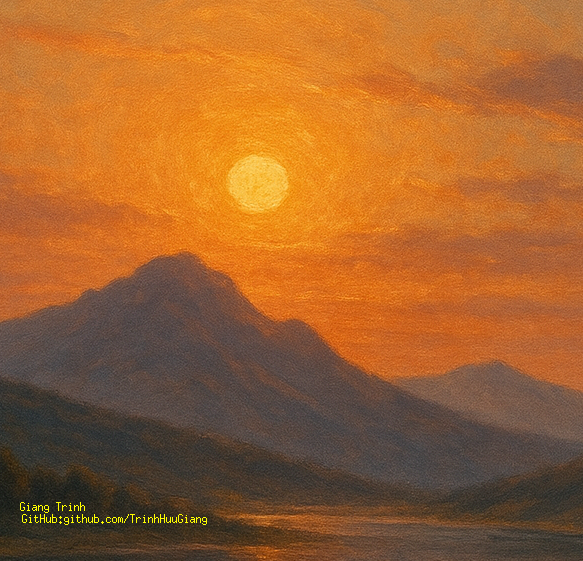
\includegraphics[width=5cm]{./sunset.png} \\
    \textbf{Hello\thanks{\LaTeX {} wikibook}}
}
% authors and groups
\author
{
    Giang Trinh\thanks{GitHub: \url{{https://github.com/TrinhHuuGiang}}}
    \and others\thanks{No one}
}
% date
\date{\today}

% draw title
\maketitle



                    % ========================================
                    % [Information pages]
                    % ========================================
%



                    % ========================================
                    % [Table of contents]
                    % ========================================
% Style for TOC, LOF, LOT
% \tocloftpagestyle{plain}
\tocloftpagestyle{headings}
% Set dot shape
\renewcommand{\cftdot}{!}
% Set dot separate distance
% it don't want dot between
% title and number set \cftnodots
% \cftnodots return 5000
% \renewcommand{\cftdotsep}{\cftnodots}
\renewcommand{\cftdotsep}{10}

% set ToC vertical space before entry
\setlength{\cftbeforepartskip}{1cm}
\setlength{\cftbeforechapskip}{2cm}
\setlength{\cftbeforesecskip}{3cm}
\setlength{\cftbeforesubsecskip}{4cm}

% set ToC indent
\setlength{\cftpartindent}{0pt}
% \setlength{\cftchapindent}{0pt}
\setlength{\cftsecindent}{30pt}
\setlength{\cftsubsecindent}{60pt}

% TOC
\hspace{0pt}
\newpage
\tableofcontents



                    % ========================================
                    % [Abbrevication pages]
                    % ========================================
\newpage
\printnomenclature



                    % ========================================
                    % [List of objects]
                    % ========================================
\newpage
\listoftables
\newpage
\listoffigures



                    % ========================================
                    % [Preface pages] 
                    % ========================================
% 



                    % ========================================
                    % [Abstract page]
                    % ========================================
% 



                                        % ========================================
                                        % [Main matter]
                                        %   - part, chapter, section ...
                                        %       are included in 7 sectioning
                                        % ========================================
% \mainmatter % only for book



                    % ========================================
                    % [Chapter 1]
                    %   Topic: 
                    % ========================================
\part{part1 title}

\chapter{chapt 1 title}

% hello \gls{qt}

\nomenclature[group 1]{Lorem 2}{Lorem paragraph 2}
\lipsum[2]


\part[Phần II: part2 title]{part2 title}

\chapter{chapt 1 title}

\section{làng tôi}

Chuyện Làng Tôi

Làng tôi nằm giữa những ngọn đồi. Phía đông là một con suối nhỏ, nước trong veo, chảy róc rách suốt ngày đêm. Mọi người trong làng đều yêu quý và giữ gìn dòng suối.

Buổi chiều, bọn trẻ thường tụ tập ở đây để chơi đá bóng. Tiếng cười, tiếng nói vang vọng cả một góc trời. Lũ chúng tôi thích nghe bà kể chuyện về những cuộc phiêu lưu của người anh hùng chống giặc ngoại xâm.

Những âm thanh của cuộc sống bình dị, của tiếng chim hót, của tiếng gà gáy, của tiếng bò gặm cỏ, đã khắc sâu vào tâm trí tôi. Nó là nguồn động lực giúp tôi cố gắng học tập. Tôi mong muốn sau này trở thành một người có ích, xây dựng quê hương giàu đẹp.

\subsection{check subsection}

à ơ ê â ư đ

% {\fontencoding{T1}\selectfont Text in T1 encoding: à ơ ê â ư đ}

% {\fontencoding{T5}\selectfont Text in T5 encoding: à ơ ê â ư đ}

\newpage

\lipsum[1] \cite{bib-unique-key}

\lipsum[2]

\lipsum[3]



            % test tikz
\newpage

\begin{center}

\setlength{\arrayrulewidth}{1mm}
\begin{tabular}[c]{|m{5cm}|m{2cm}|m{3cm}|}
    \hline
    \hspace{0pt}\newline
    \begin{tikzpicture}
        \draw (-15pt,0pt) -- (15pt,0pt);
        \draw (0,-1.5) -- (0,1.5);
    \end{tikzpicture}
    &  &
    This a cross inside a `fcolorbox'\\[\the\dimexpr\baselineskip/2\relax]
    % \cline{2-2} % above \\[-1mm] % move next row higher 1mm 
    \hline

\end{tabular}

\end{center}

this is \the\dimexpr-\baselineskip/2\relax



                                        % ========================================
                                        % [Back matter]
                                        %   - appendix, glossary, bibliograpy, index
                                        % ========================================
% \backmatter % only for book

                                        


                    % ========================================
                    % [Appendix]
                    % ========================================
\appendix

\chapter{Append 1}

                    % ========================================
                    % [Glossary]
                    % ========================================
% Glossary
\printglossaries



                    % ========================================
                    % [Bibliograpy]
                    % ========================================
% other bibliography style 
\bibliographystyle{ieeetr}
% \bibliographystyle{plain}
% register `.bib` file and print with style
% \bibliography{sample_bib_1,sample_bib_2,...,samplen} 
\bibliography{bibli_test} 



                    % ========================================
                    % [Index]
                    % ========================================
% indexing
\printindex



% ========================================
% End Document
% ========================================
\end{document}
